\chapter{SYSTEM INTERFACE AND PHYSICAL DESIGN}
\label{chap:system_interface_physical_design}

In the software development lifecycle, the system interface and physical design phase translates the static logical structures and dynamic workflows into physical components that are directly usable by human actors and compile-ready for database servers \cite{system_design_roadmap}. While use cases and sequence diagrams detail functional boundaries and message routing paths, this chapter focuses on the design of the user interfaces (UI) and the physical database layout. The user interface design establishes the visual viewport, navigational controls, input fields, and feedback mechanisms that shape the user experience (UX) for students and teachers. Simultaneously, the physical database design defines the concrete SQL schemas, column types, lengths, constraints, and relational indexes required to store and query telemetry data, exam configurations, and grading results securely and efficiently. By mapping both the interactive front-end layouts and the persistent back-end storage schemas, the physical design guarantees that the software prototype remains secure, performant, and resilient under real-world lab conditions.

\section{System User Interfaces}
A system user interface (UI) represents the graphical and interactive gateway through which human users interact with software systems. The UI establishes how buttons, text forms, selection toggles, tables, and charts are arranged, ensuring that users can execute tasks efficiently without cognitive overload \cite{user_interface_guide}. In the SmartExam platform, the UI design is divided into two distinct clients: a native Windows WPF desktop client for student exam execution and a responsive React web dashboard for instructor supervision and evaluation. The design prioritizes visual clarity, clean layouts, and responsive components, adhering to modern UI/UX guidelines such as accessibility, clear warnings, and real-time state updates. By maintaining consistency in color palettes, typography, and controls, the platform minimizes usability errors during exams and supports seamless coordination between invigilators and candidates.

The interfaces detailed below cover the user views of the completed platform modules, displaying the operational layouts for candidate authentication, device binding, diagnostics checks, secure workspace lockdown, proctoring dashboards, live telemetry monitors, and compiler results.

\subsection{Student Login and Device Binding Interface}
The student login interface verifies student credentials and queries native Windows APIs to generate and compare Hardware ID (HWID) hashes, preventing unauthorized workstation proxy attempts. The login page layout is illustrated in Figure~\ref{fig:ui_student_login}.

\begin{figure}[H]
\centering
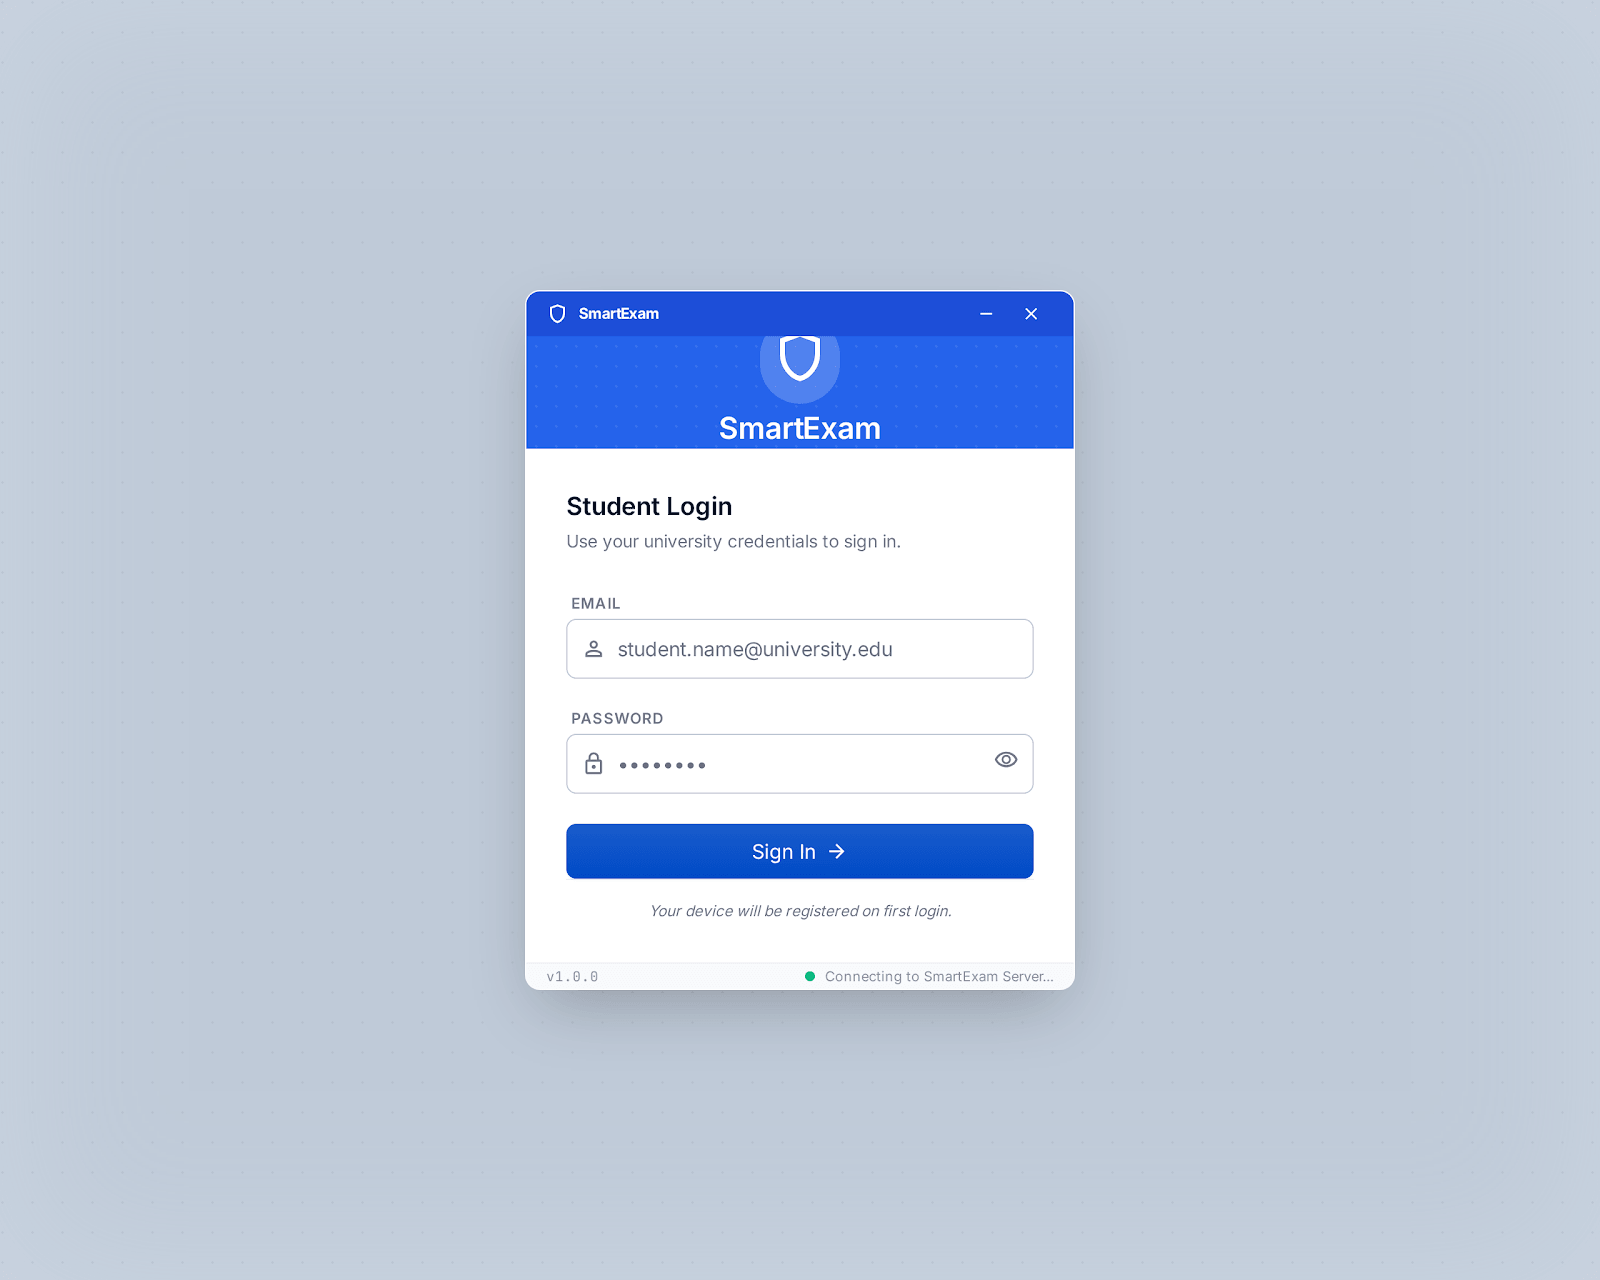
\includegraphics[width=0.7\linewidth]{Figures/ui_student_login.png}
\caption{WPF Student Client Login and Device Verification Interface}
\label{fig:ui_student_login}
\end{figure}

\subsection{Pre-Exam Workstation Diagnostics Interface}
The pre-exam diagnostics interface runs automated webcam, microphone, network connectivity, and running background process compliance scans before granting candidate access to the exam. The diagnostics verification checklist layout is shown in Figure~\ref{fig:ui_student_diagnostics}.

\begin{figure}[H]
\centering
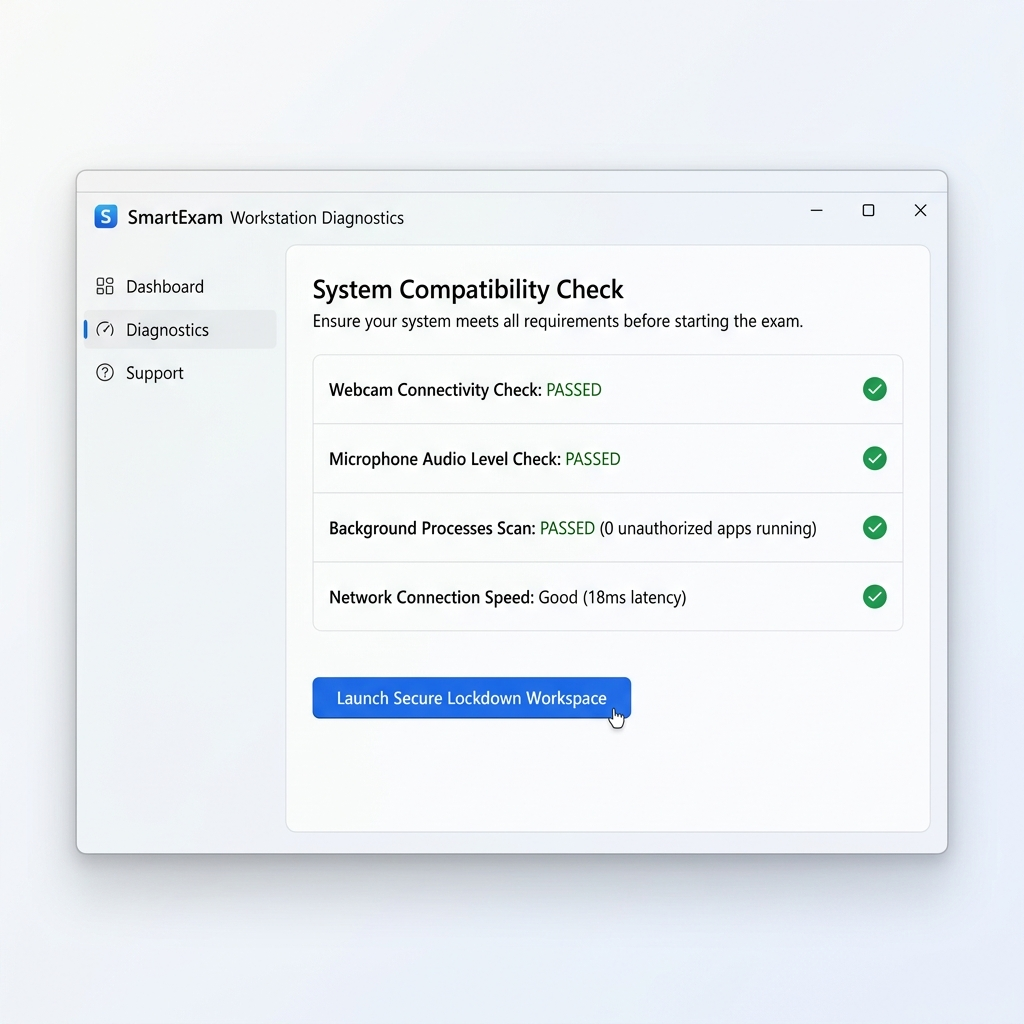
\includegraphics[width=0.7\linewidth]{Figures/ui_student_diagnostics.png}
\caption{WPF Student Client Pre-Exam System Diagnostics Interface}
\label{fig:ui_student_diagnostics}
\end{figure}

\subsection{Student Exam Lockdown Workspace}
The student exam lockdown workspace enforces fullscreen restrictions, disables secondary monitor outputs, blocks keyboard task-switching shortcuts, and provides rich-text editors for candidate responses. The locked exam client workspace layout is shown in Figure~\ref{fig:ui_student_workspace}.

\begin{figure}[H]
\centering
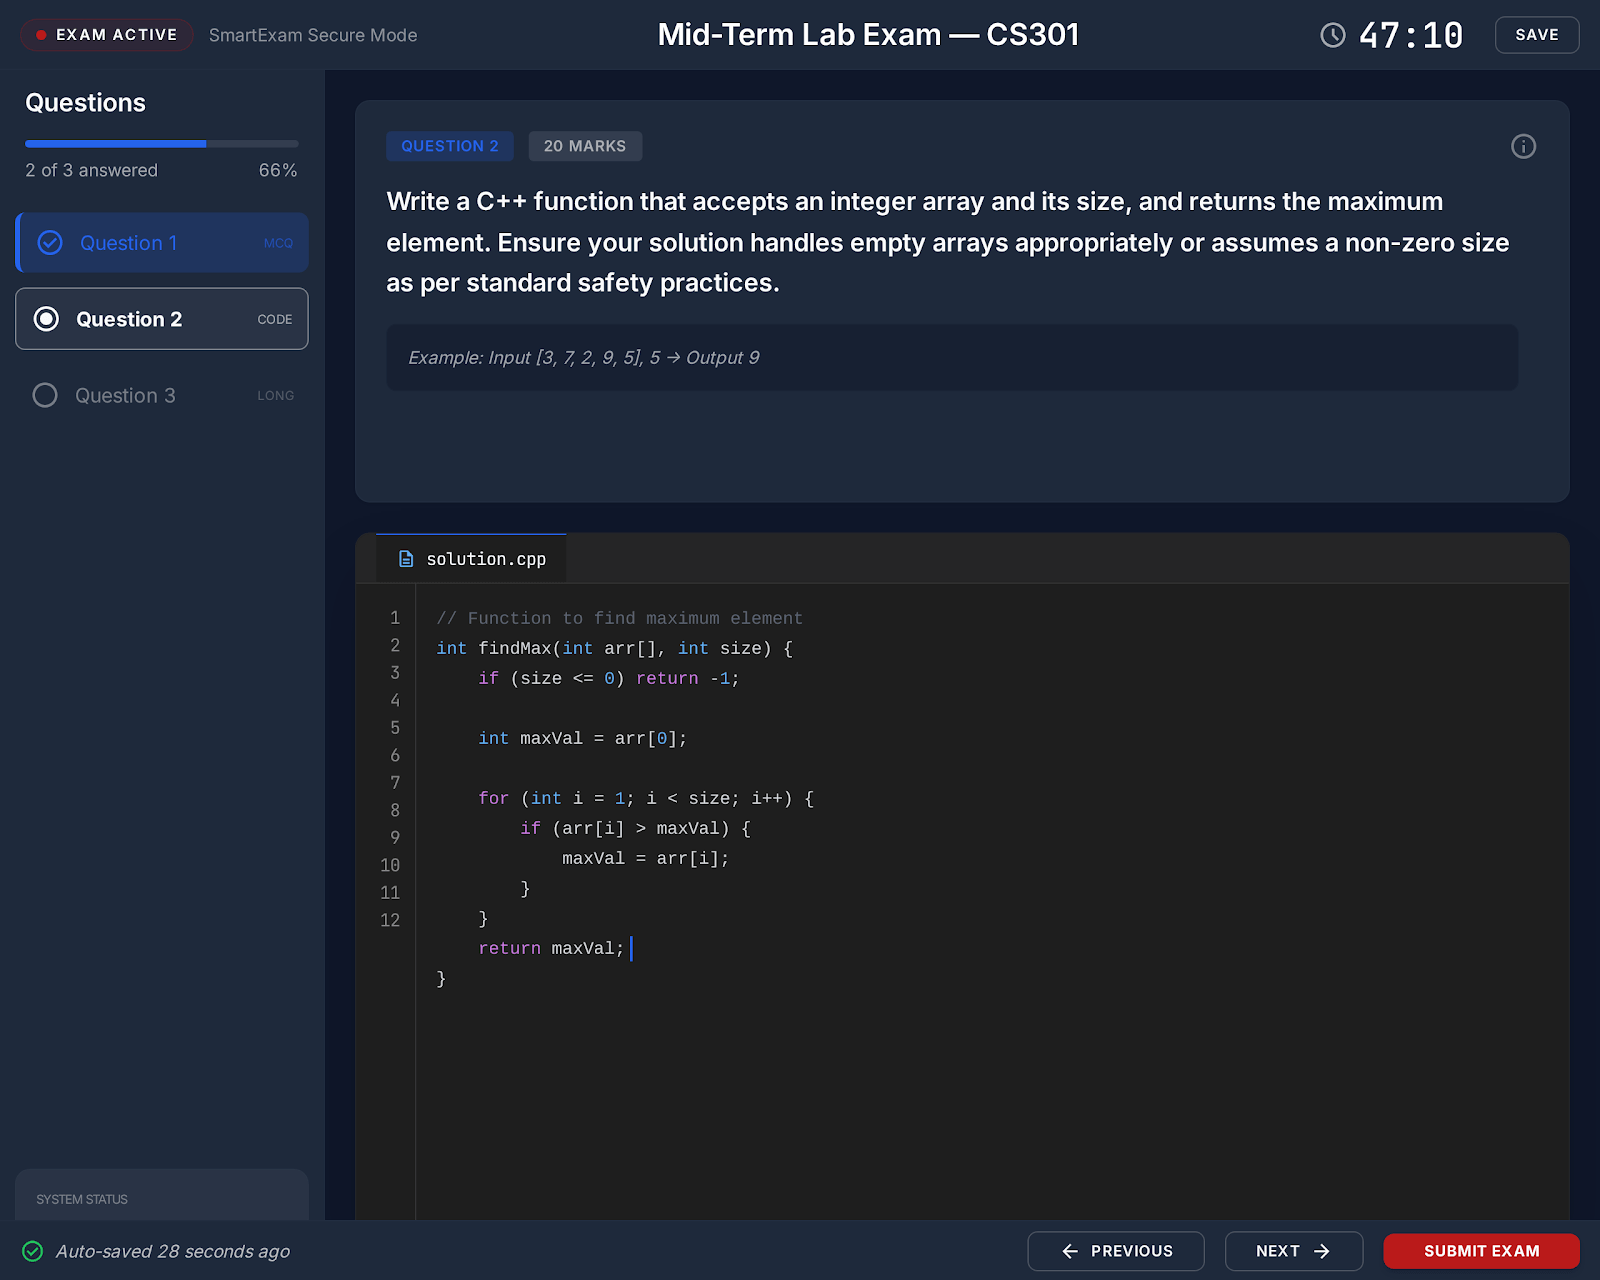
\includegraphics[width=0.7\linewidth]{Figures/ui_student_workspace.png}
\caption{WPF Student Client Active Exam Lockdown Workspace}
\label{fig:ui_student_workspace}
\end{figure}

\subsection{Teacher Proctoring Dashboard Overview}
The teacher dashboard overview console displays room statistics, active exam listings, pending hardware unbinding requests, and quick navigation controls for instructors. The web panel overview layout is illustrated in Figure~\ref{fig:ui_teacher_dashboard}.

\begin{figure}[H]
\centering
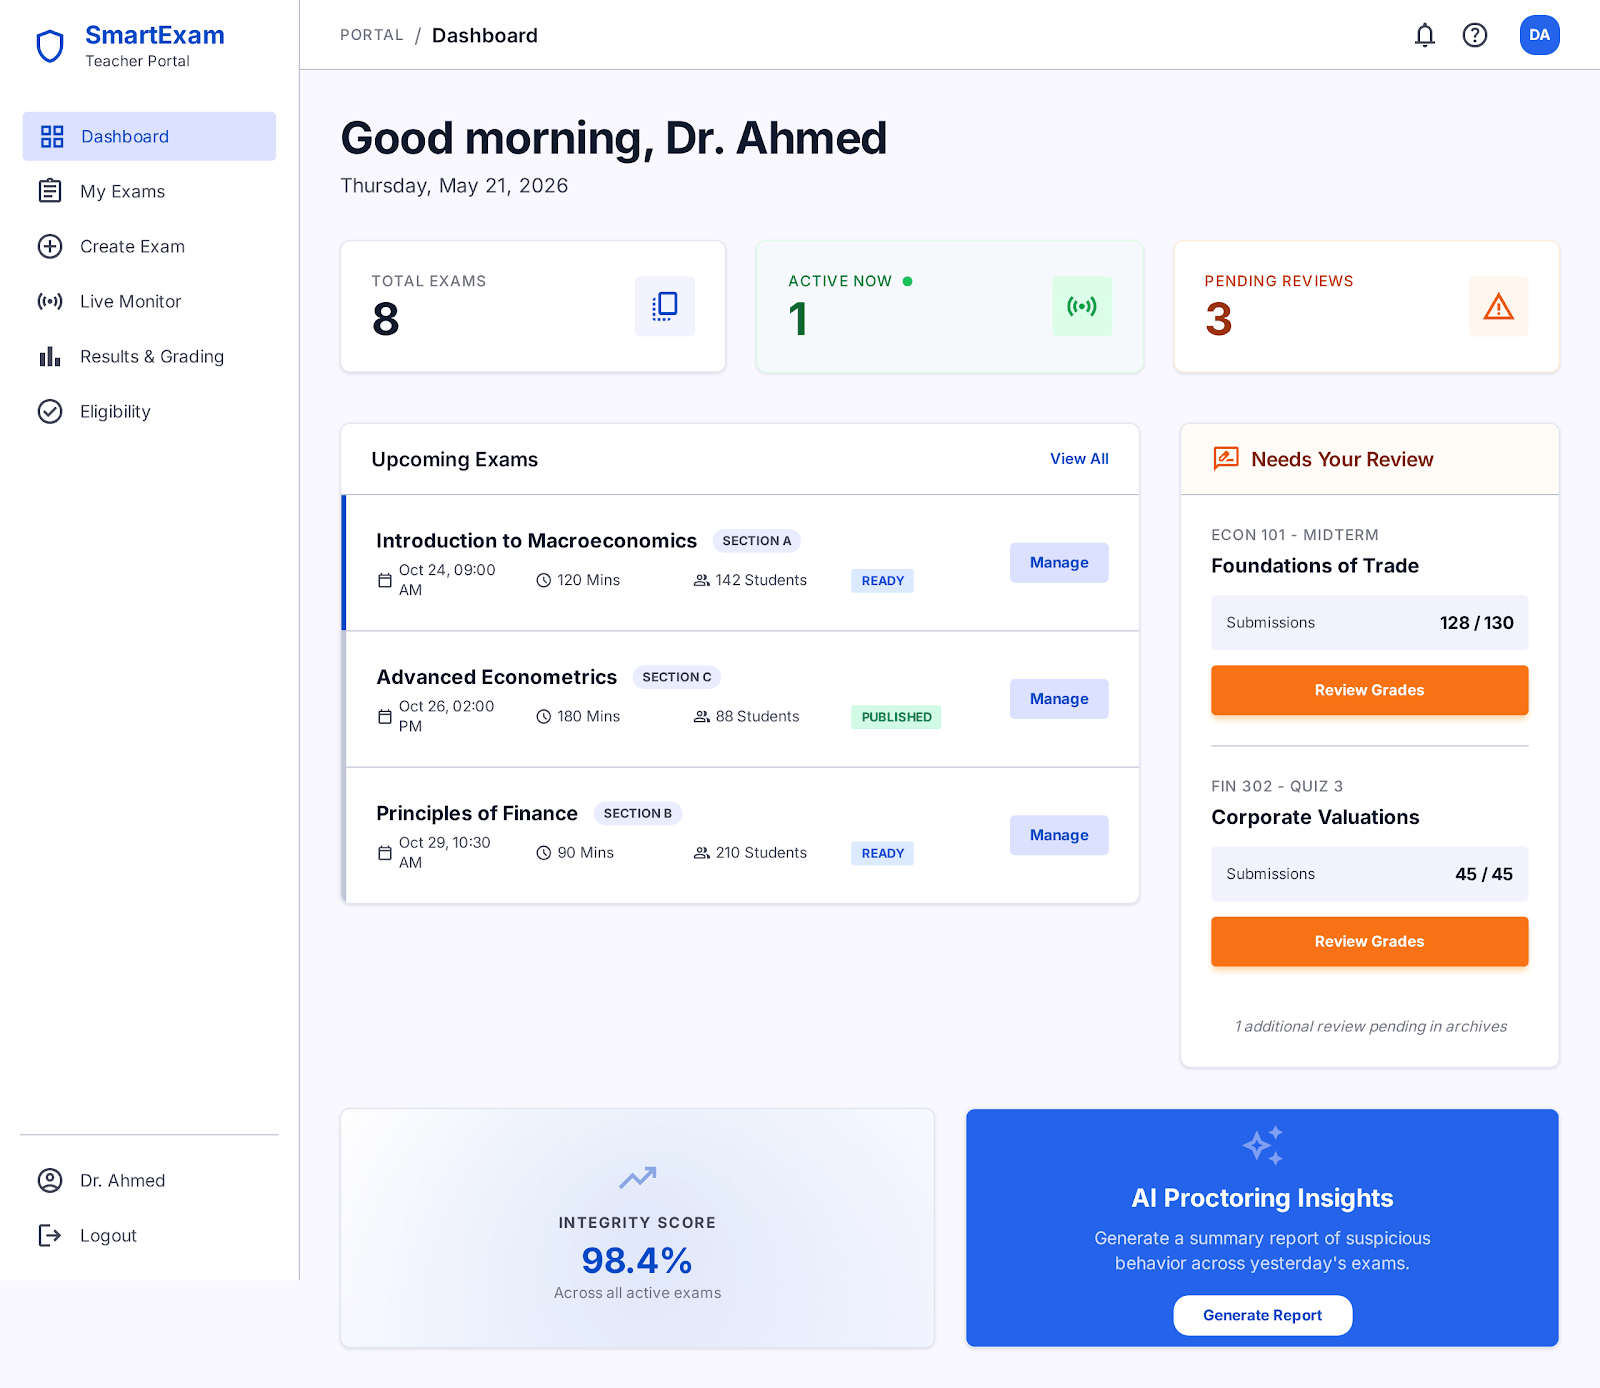
\includegraphics[width=0.7\linewidth]{Figures/ui_teacher_dashboard.png}
\caption{React Web Panel Teacher Dashboard Overview Interface}
\label{fig:ui_teacher_dashboard}
\end{figure}

\subsection{Live Telemetry Ingestion and Monitoring Interface}
The live telemetry proctoring interface displays color-coded student status cards, webcam snapshots, process lists, and focus timelines streamed over persistent WebSocket connections. The proctoring grid and override panel are shown in Figure~\ref{fig:ui_teacher_live_monitoring}.

\begin{figure}[H]
\centering
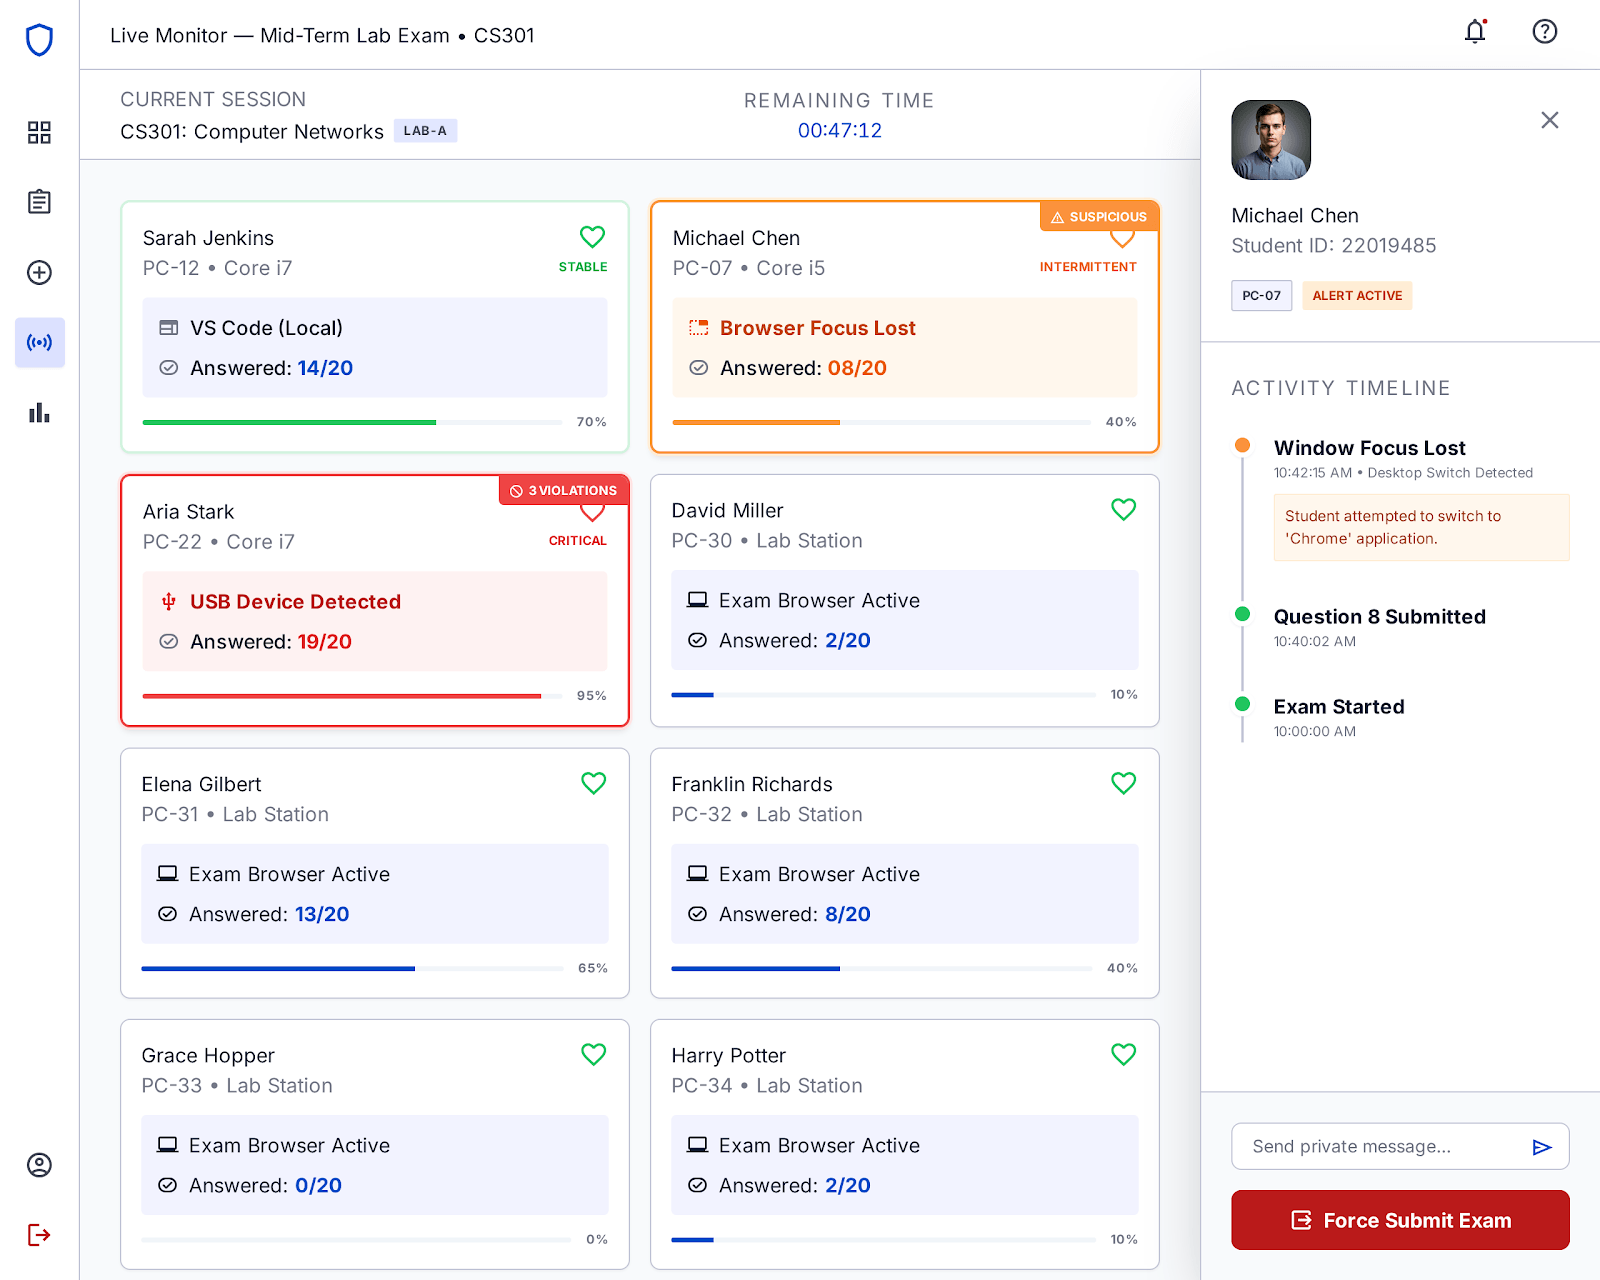
\includegraphics[width=0.7\linewidth]{Figures/ui_teacher_live_monitoring.png}
\caption{React Web Panel Live Telemetry Proctoring and Alerts Dashboard}
\label{fig:ui_teacher_live_monitoring}
\end{figure}

\subsection{Code Compilation and AI Evaluation Panel}
The code compilation panel details Docker compilation outcomes, test case pass percentages, sentence-transformers semantic similarity scores, and class-wide plagiarism analysis. The automated grading dashboard layout is illustrated in Figure~\ref{fig:ui_teacher_ai_grading}.

\begin{figure}[H]
\centering
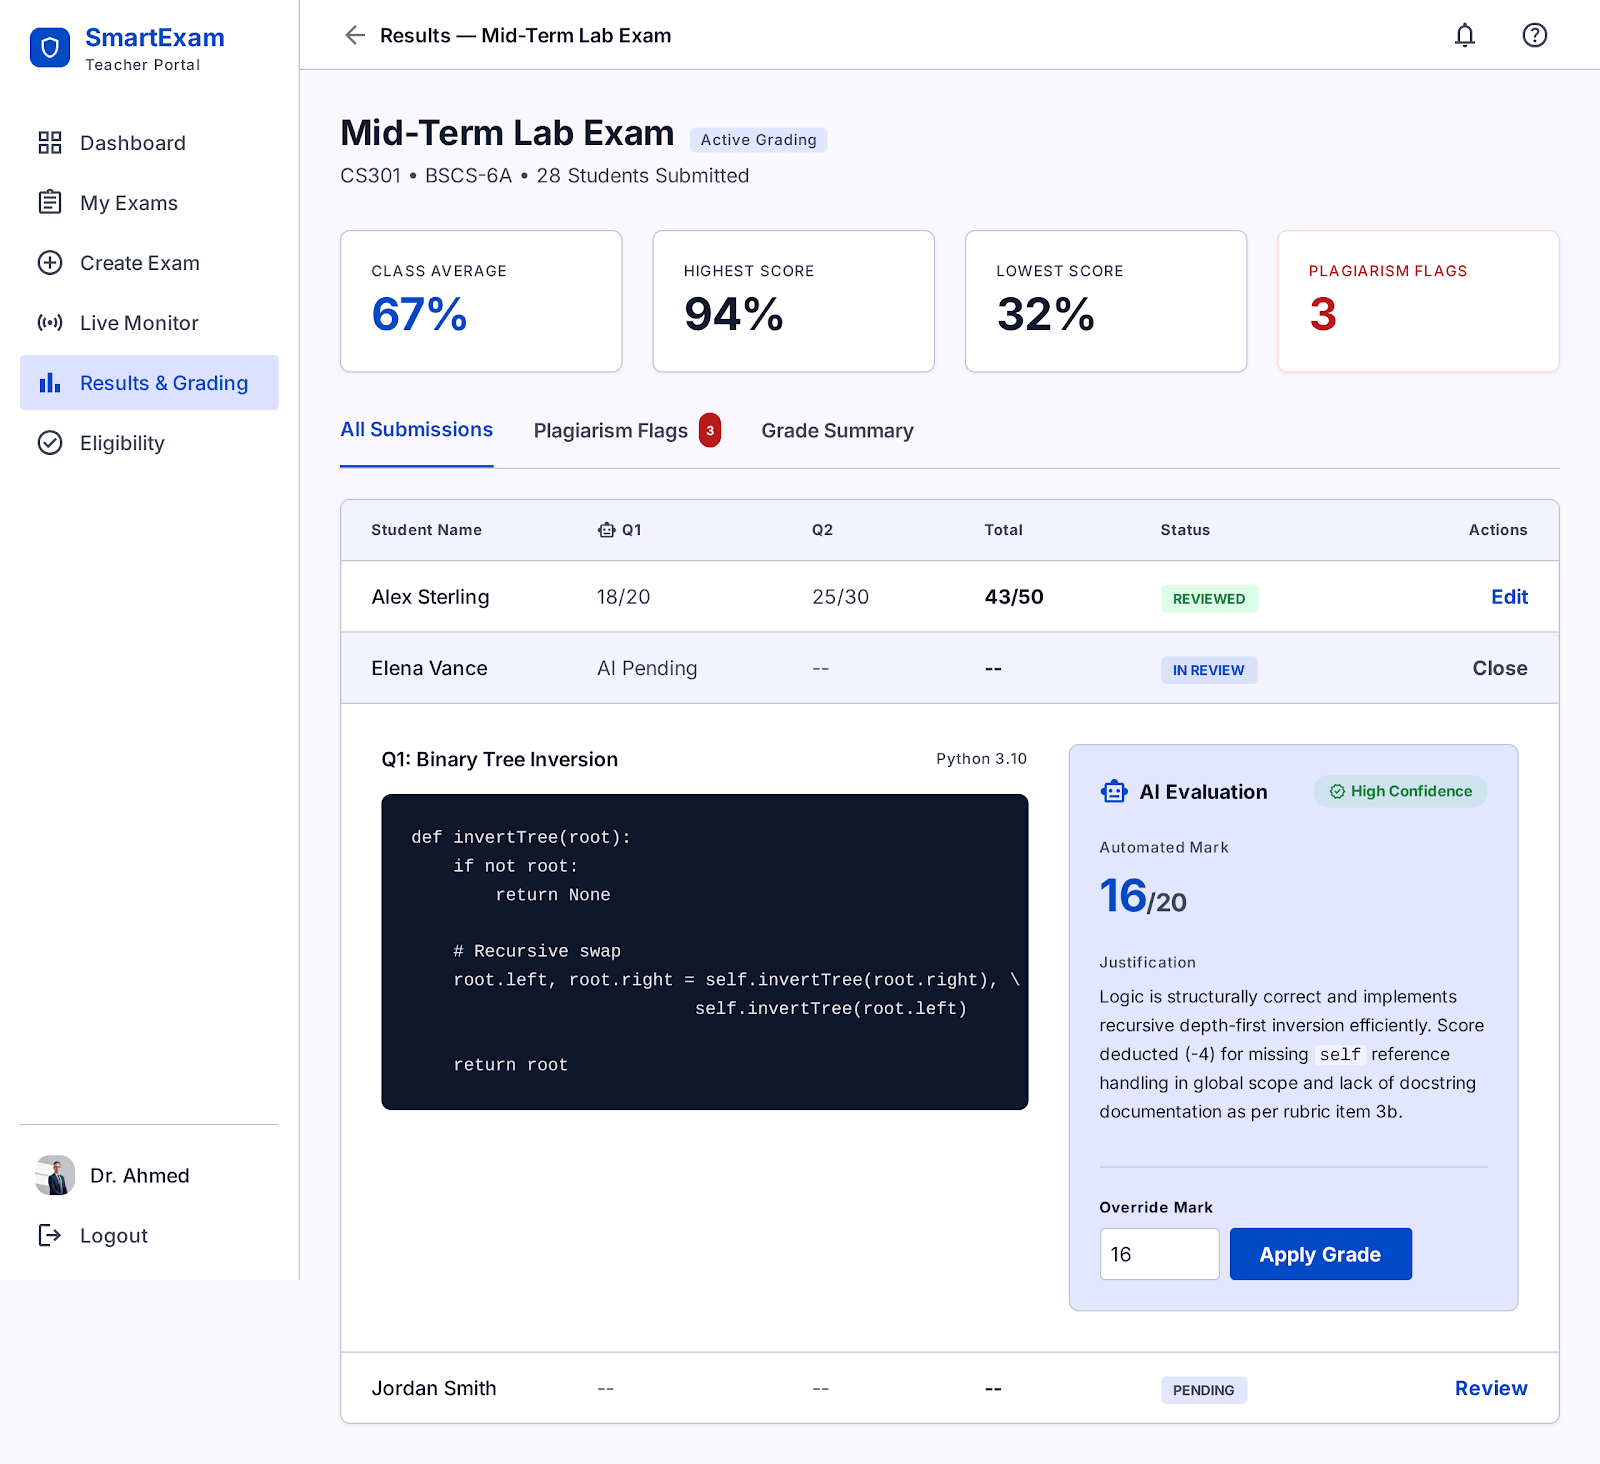
\includegraphics[width=0.7\linewidth]{Figures/ui_teacher_ai_grading.png}
\caption{React Web Panel Automated Code Evaluation and Plagiarism Panel}
\label{fig:ui_teacher_ai_grading}
\end{figure}

\subsection{Labs and Workstations Seating Map Interface}
The seating map interface maps candidate logins to laboratory seat coordinates and configures network IP filters to restrict access to physical exam rooms. The lab terminal configuration grid is shown in Figure~\ref{fig:ui_labs_workstations}.

\begin{figure}[H]
\centering
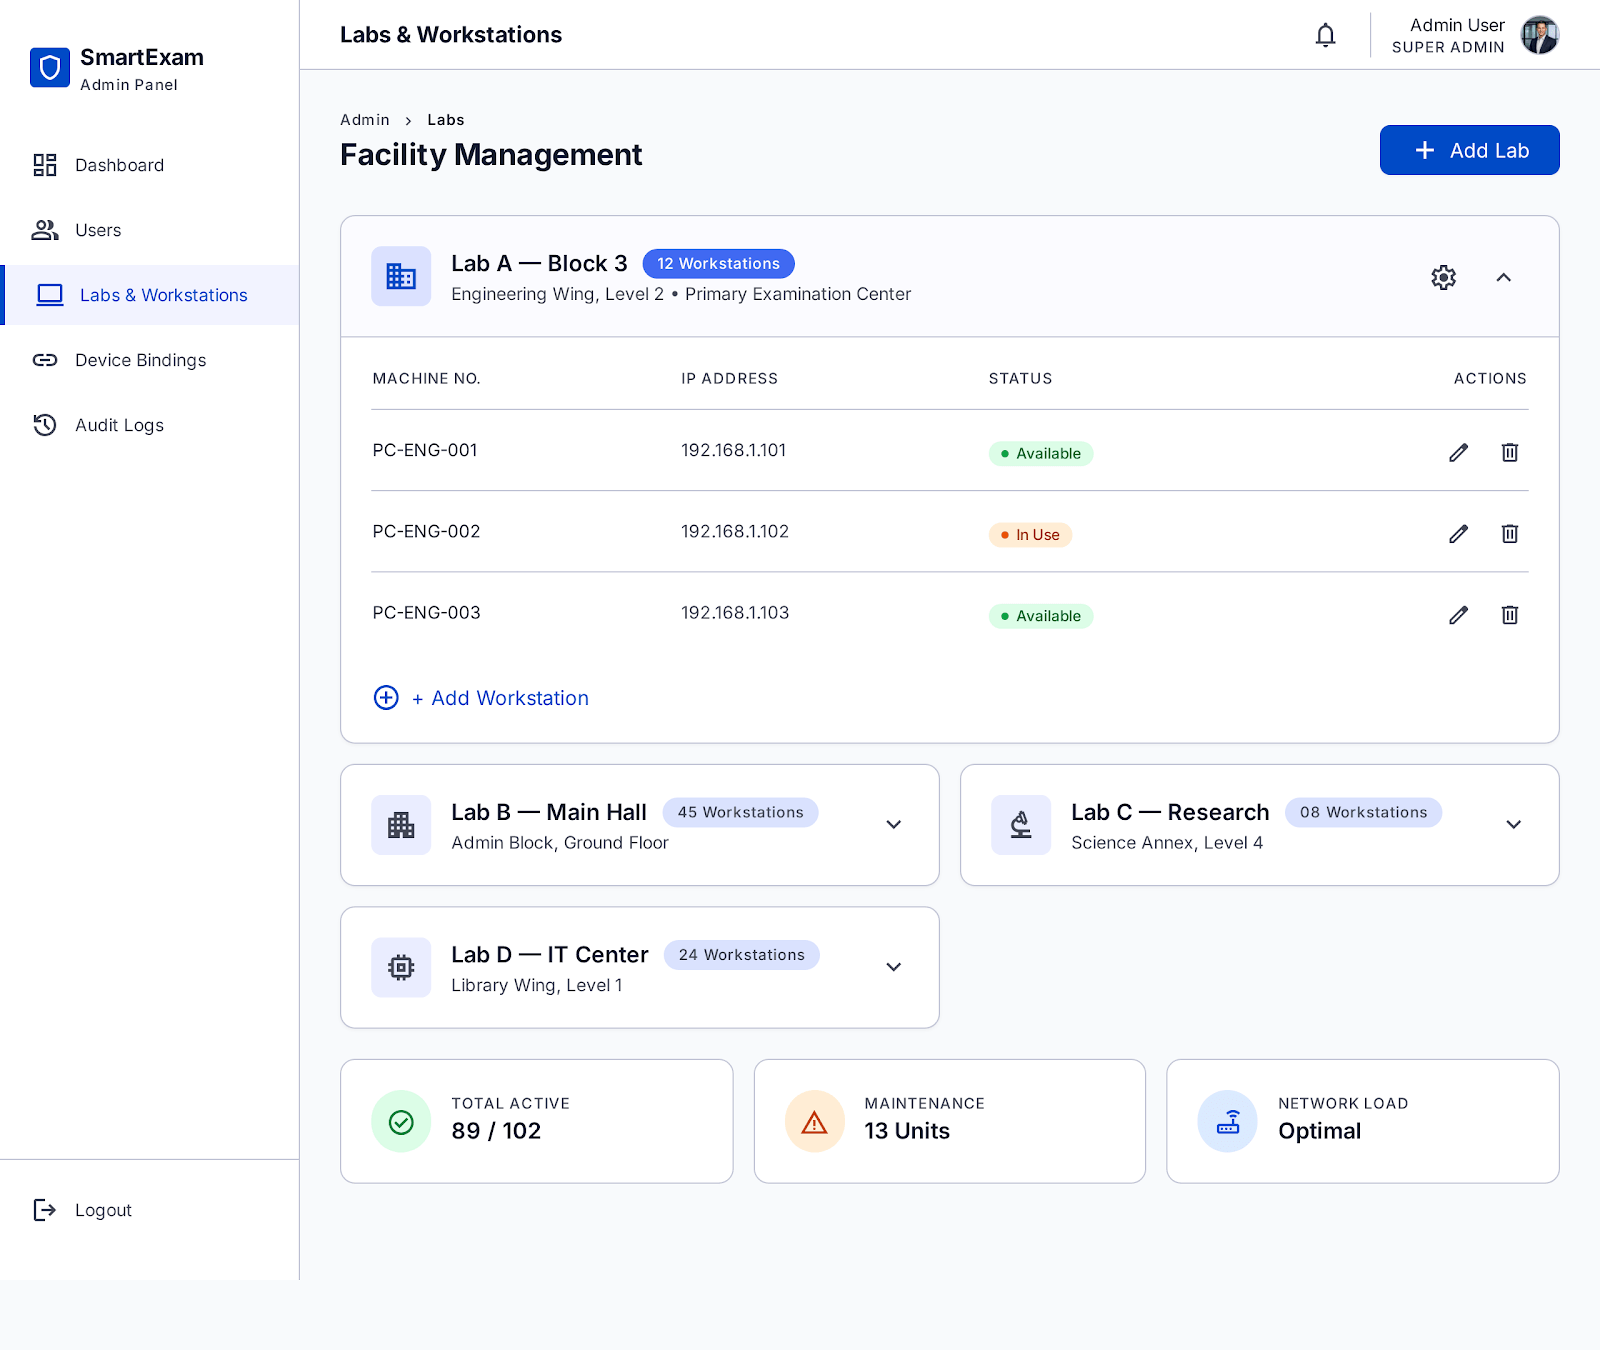
\includegraphics[width=0.7\linewidth]{Figures/ui_labs_workstations.png}
\caption{React Web Panel Labs and Workstations Seating Configuration Interface}
\label{fig:ui_labs_workstations}
\end{figure}

\subsection{Device Bindings and Hardware Identifier Interface}
The device bindings interface logs CPU and motherboard HWID bindings, allowing administrators to audit machine allocations and approve workstation override requests. The HWID management panel is illustrated in Figure~\ref{fig:ui_device_bindings}.

\begin{figure}[H]
\centering
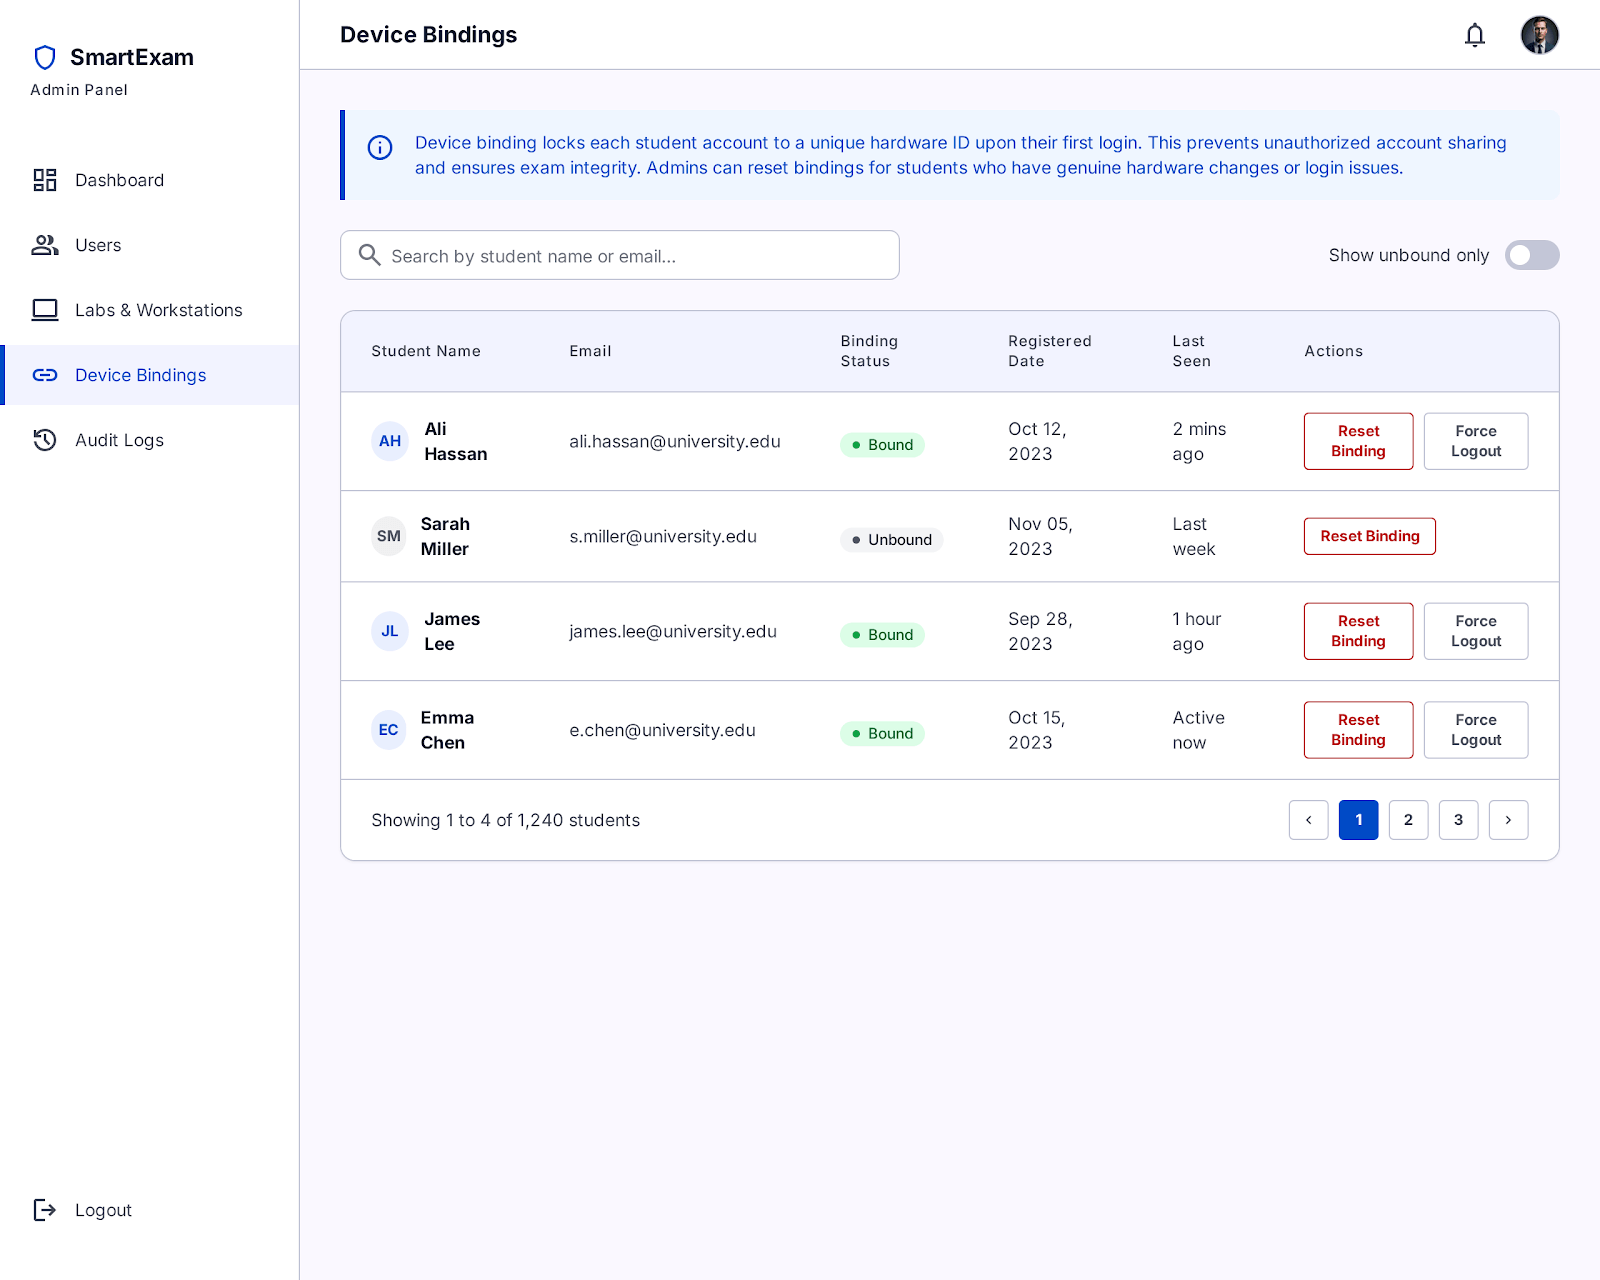
\includegraphics[width=0.7\linewidth]{Figures/ui_device_bindings.png}
\caption{React Web Panel Device Bindings and HWID Management Interface}
\label{fig:ui_device_bindings}
\end{figure}

\subsection{Student Performance and Analytics Dashboard}
The student portal dashboard renders candidate grading reports, automated feedback, performance average comparison charts, and flagged telemetry alert summaries. The candidate results panel is shown in Figure~\ref{fig:ui_student_performance}.

\begin{figure}[H]
\centering
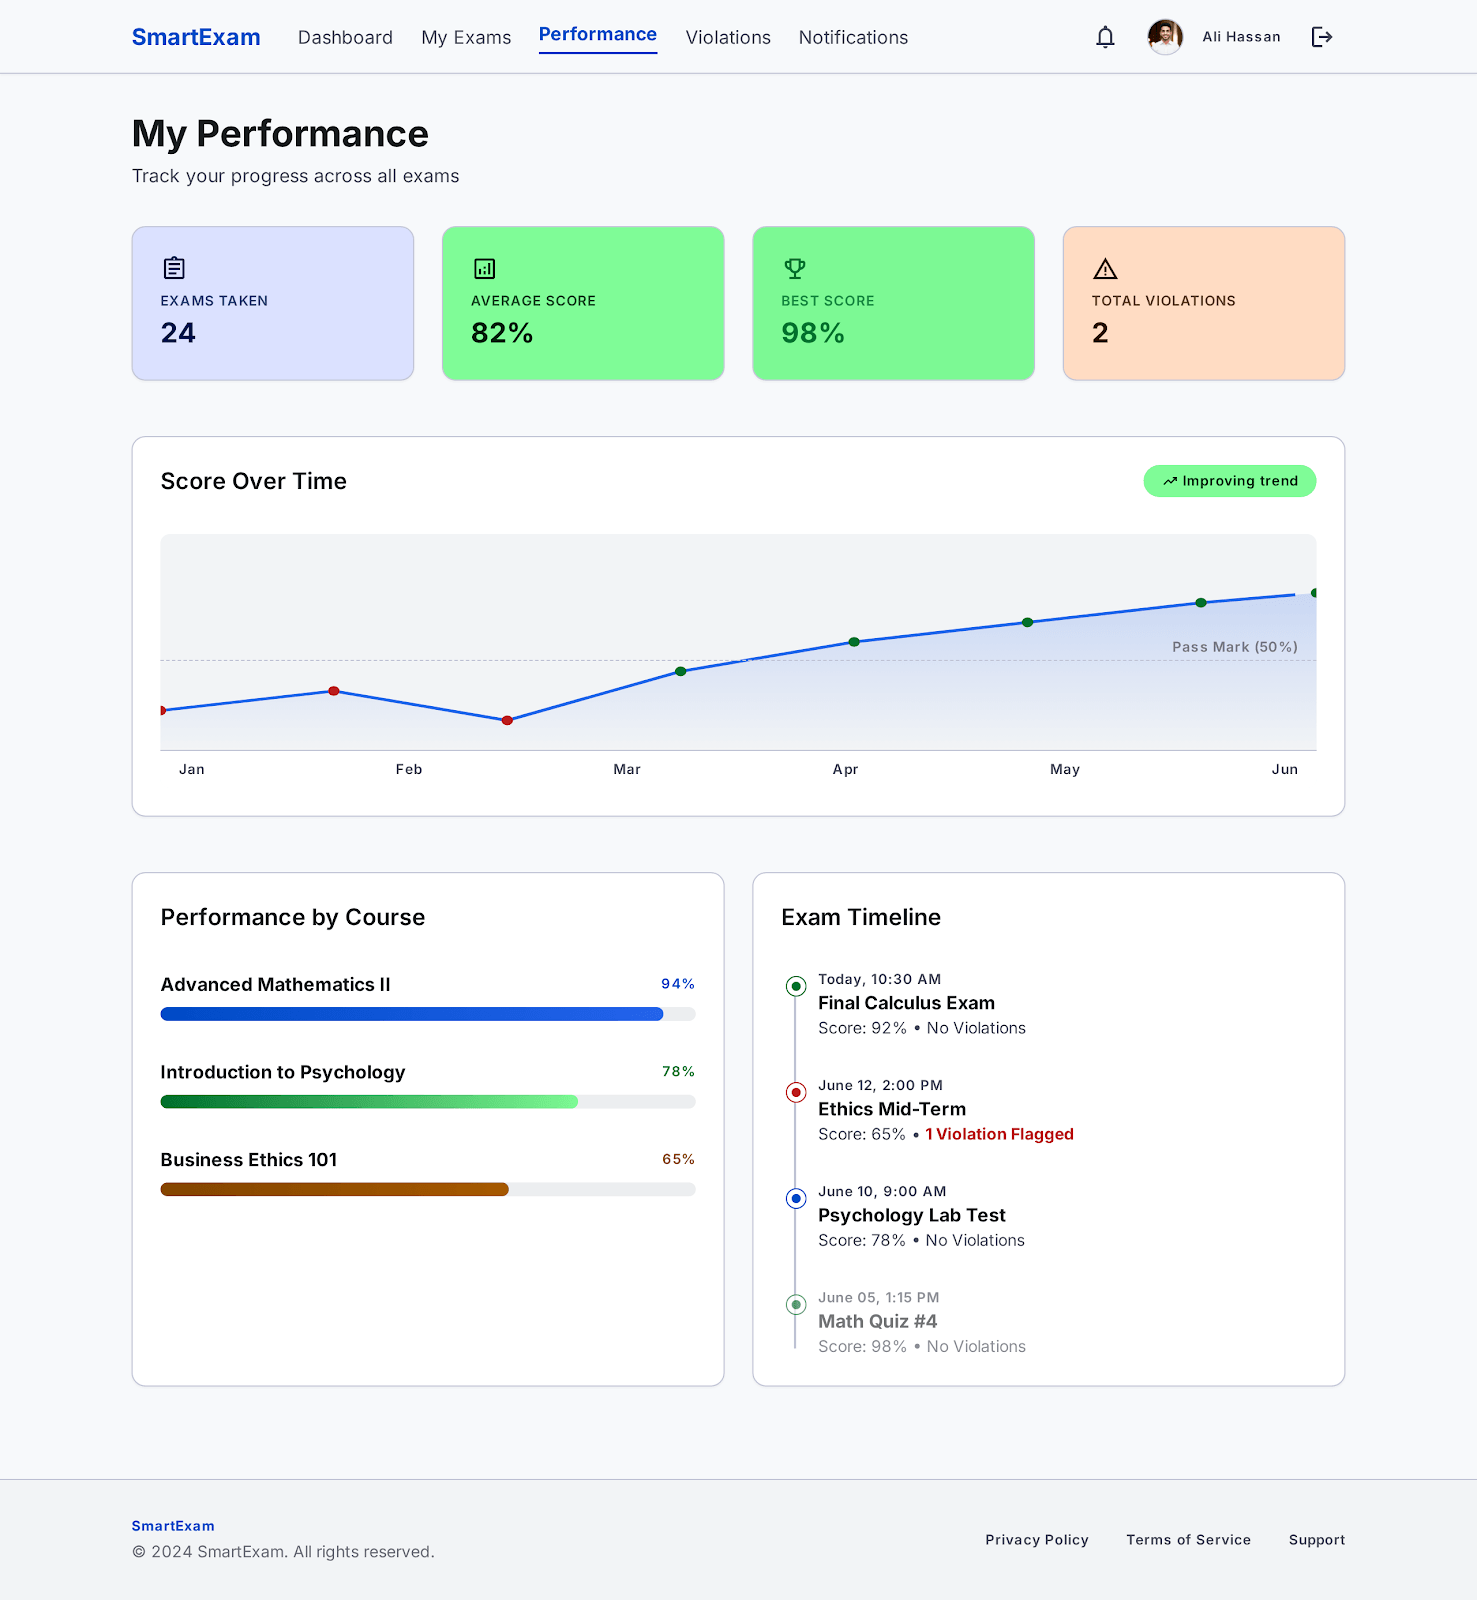
\includegraphics[width=0.7\linewidth]{Figures/ui_student_performance.png}
\caption{React Web Student Portal Performance and Analytics Dashboard}
\label{fig:ui_student_performance}
\end{figure}

\subsection{Security Audit Logs Interface}
The security audit logs interface records administrator override actions, role changes, and system settings updates in an immutable, read-only ledger for verification. The admin transaction log interface is illustrated in Figure~\ref{fig:ui_audit_logs}.

\begin{figure}[H]
\centering
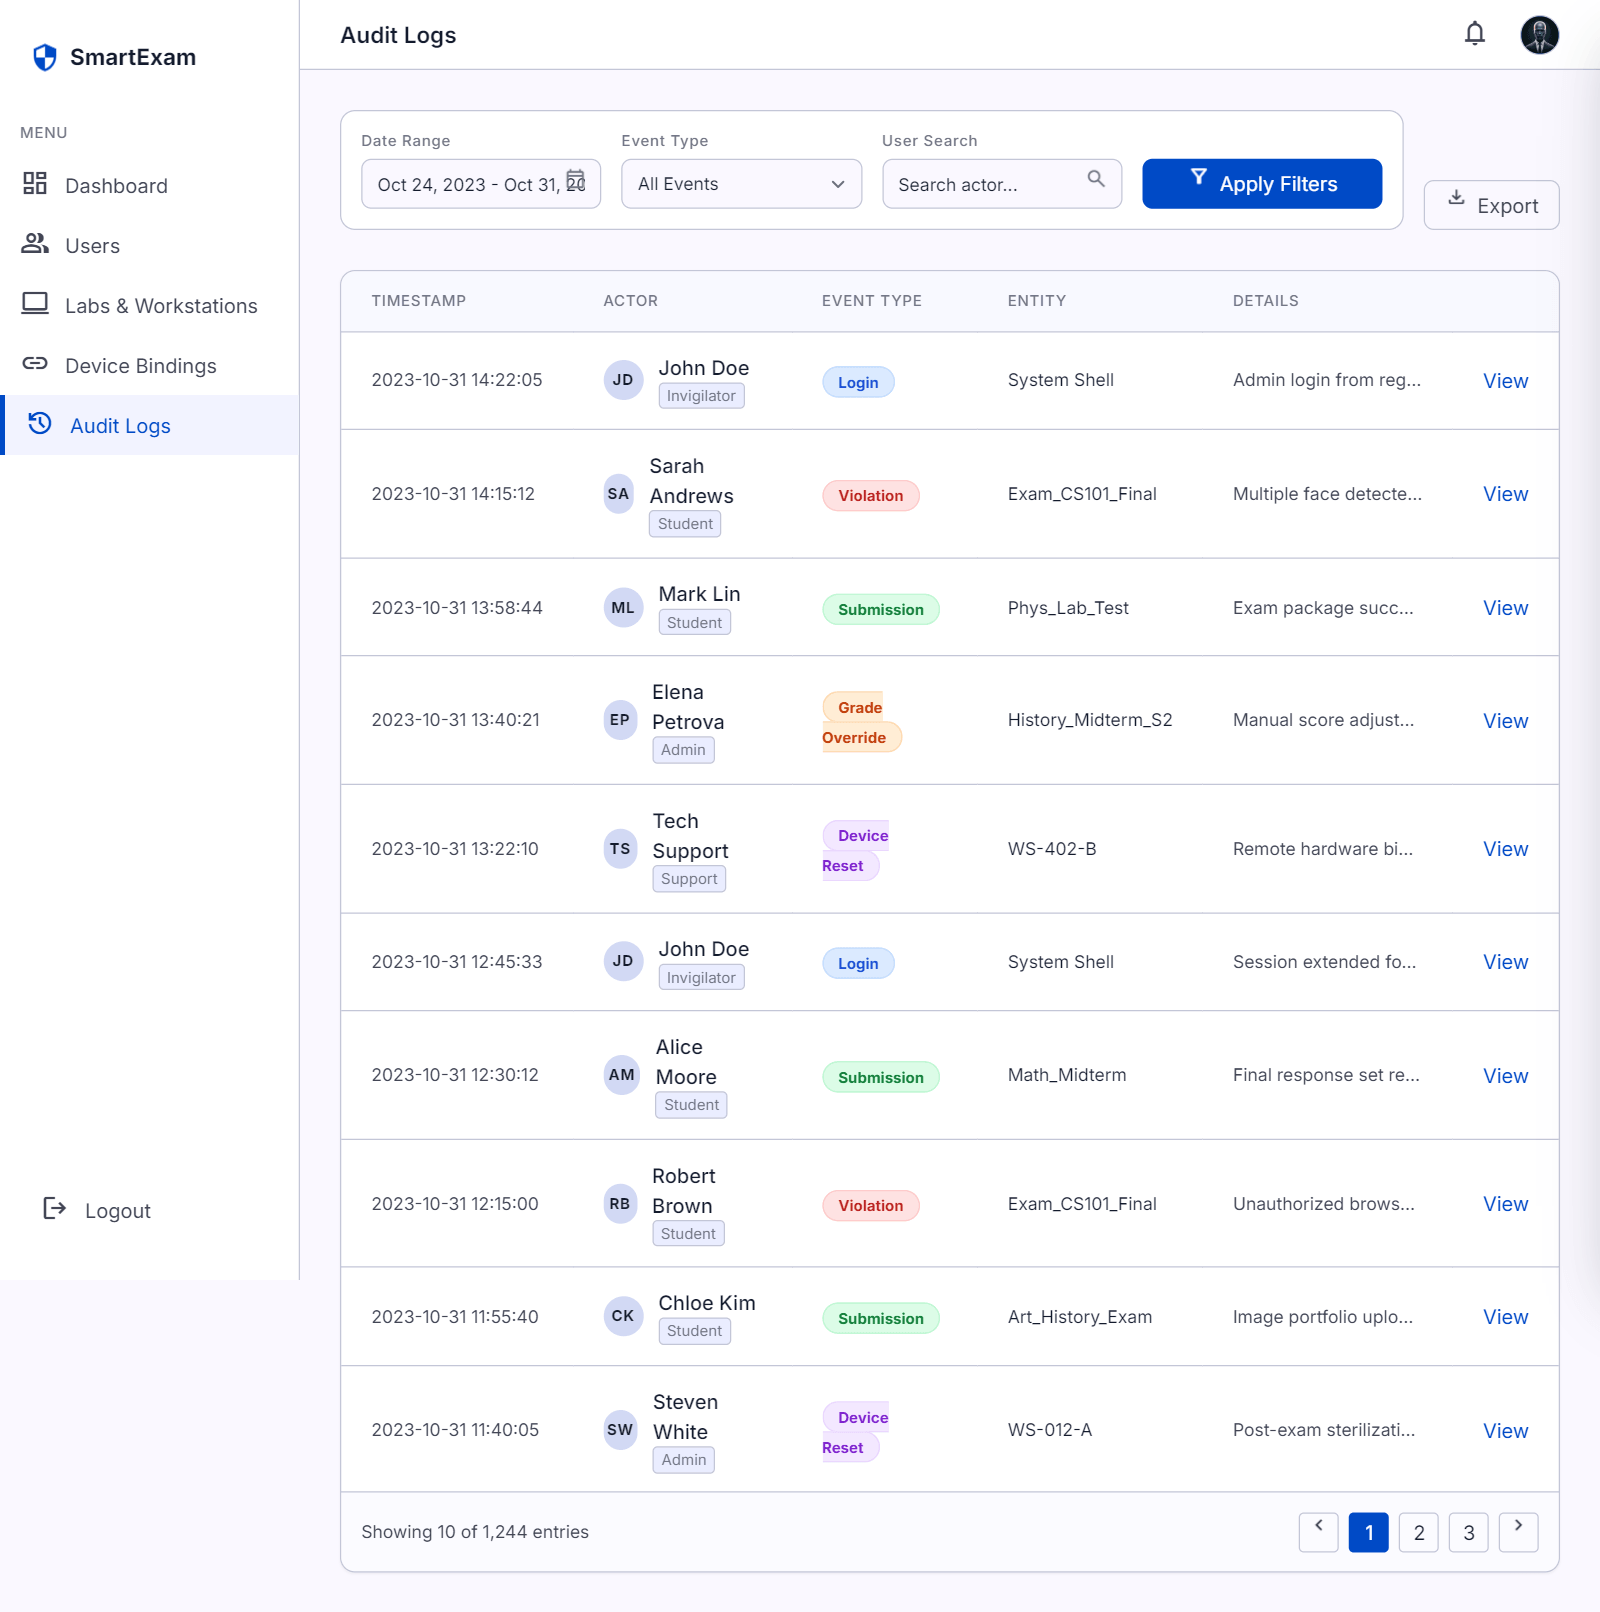
\includegraphics[width=0.7\linewidth]{Figures/ui_audit_logs.png}
\caption{React Web Panel System Security Audit Logs Interface}
\label{fig:ui_audit_logs}
\end{figure}


\section{Physical Database Tables}
Physical database design translates the logical Entity Relationship Diagram (ERD) into actual relational SQL tables implemented on the Neon PostgreSQL platform. This stage involves defining table columns, data types (e.g., \texttt{SERIAL}, \texttt{VARCHAR}, \texttt{TIMESTAMP}), lengths, nullable/non-nullable constraints, primary key bounds, and foreign key relations. Proper physical design ensures data integrity, prevents redundant records, and supports quick data retrieval. In the SmartExam database, columns that are frequently filtered or joined are indexed, and foreign keys are configured with explicit cascading actions to maintain consistency across tables \cite{users_table_budibase}. 

Below are the physical schema table specifications for the fourteen database tables of the SmartExam system, structured using the required double-hline format.

\subsection{Roles Table (Roles)}
The \texttt{Roles} table defines the user access levels within the application, such as Administrator, Teacher, or Student, mapping capabilities to explicit roles. The physical database schema for the roles table is defined in Table~\ref{tab:roles_table}.

\begin{table}[H]
\centering
\caption{Physical Database Schema for User Roles (Roles)}
\label{tab:roles_table}
\renewcommand{\arraystretch}{1.2}
\begin{tabular}{l|ccccc}
\hline\hline
\textbf{Field Name} & \textbf{Description} & \textbf{Type} & \textbf{Length} & \textbf{Default} & \textbf{Not Null} \\ \hline\hline
Id & Auto-incrementing identifier & Serial & - & PK & Yes \\
RoleName & Name of the user permission role & Varchar & 50 & - & Yes \\
\hline\hline
\end{tabular}
\end{table}

\subsection{Users Table (Users)}
The \texttt{Users} table manages the main profile accounts for students, instructors, and administrators. It links email credentials, encrypted BCrypt password hashes, names, and role identifiers together. The physical database schema for the users table is defined in Table~\ref{tab:users_table}.

\begin{table}[H]
\centering
\caption{Physical Database Schema for User Accounts (Users)}
\label{tab:users_table}
\renewcommand{\arraystretch}{1.2}
\begin{tabular}{l|ccccc}
\hline\hline
\textbf{Field Name} & \textbf{Description} & \textbf{Type} & \textbf{Length} & \textbf{Default} & \textbf{Not Null} \\ \hline\hline
Id & Auto-incrementing identifier & Serial & - & PK & Yes \\
Email & Primary user contact and login email & Varchar & 100 & - & Yes \\
PasswordHash & BCrypt encrypted credentials hash & Varchar & 255 & - & Yes \\
FullName & Full legal name of the user & Varchar & 100 & - & Yes \\
RoleId & Foreign key referencing Roles table & Integer & - & - & Yes \\
CreatedAt & Timestamp when account was created & Timestamp & - & NOW() & Yes \\
\hline\hline
\end{tabular}
\end{table}

\subsection{Device Bindings Table (DeviceBindings)}
The \texttt{DeviceBindings} table binds student accounts to specific hardware configs using CPU and motherboard HWID hashes, establishing a one-to-one link. The physical database schema for the device bindings table is detailed in Table~\ref{tab:device_bindings_table}.

\begin{table}[H]
\centering
\caption{Physical Database Schema for Device Bindings (DeviceBindings)}
\label{tab:device_bindings_table}
\renewcommand{\arraystretch}{1.2}
\begin{tabular}{l|ccccc}
\hline\hline
\textbf{Field Name} & \textbf{Description} & \textbf{Type} & \textbf{Length} & \textbf{Default} & \textbf{Not Null} \\ \hline\hline
Id & Auto-incrementing identifier & Serial & - & PK & Yes \\
UserId & Foreign key referencing Users table & Integer & - & Unique & Yes \\
HWID & Unique hashed hardware identifier & Varchar & 255 & Unique & Yes \\
DeviceDetails & Device motherboard and CPU model text & Text & - & - & No \\
BoundAt & Timestamp when binding was established & Timestamp & - & NOW() & Yes \\
\hline\hline
\end{tabular}
\end{table}

\subsection{Exams Table (Exams)}
The \texttt{Exams} table acts as the configuration store for assessments, tracking titles, question sets, whitelist processes, duration limits, and timestamps. The physical database schema for the exams table is specified in Table~\ref{tab:exams_table}.

\begin{table}[H]
\centering
\caption{Physical Database Schema for Exams (Exams)}
\label{tab:exams_table}
\renewcommand{\arraystretch}{1.2}
\begin{tabular}{l|ccccc}
\hline\hline
\textbf{Field Name} & \textbf{Description} & \textbf{Type} & \textbf{Length} & \textbf{Default} & \textbf{Not Null} \\ \hline\hline
Id & Auto-incrementing identifier & Serial & - & PK & Yes \\
Title & Title header of the exam & Varchar & 100 & - & Yes \\
Description & Explanatory instructions for candidates & Text & - & - & No \\
Duration & Time duration limit in minutes & Integer & - & - & Yes \\
StartTime & Scheduled opening timestamp & Timestamp & - & - & Yes \\
EndTime & Scheduled closing timestamp & Timestamp & - & - & Yes \\
IsActive & Flag indicating exam accessibility & Boolean & - & False & Yes \\
CreatedBy & Foreign key referencing Users table & Integer & - & - & Yes \\
\hline\hline
\end{tabular}
\end{table}

\subsection{Questions Table (Questions)}
The \texttt{Questions} table stores the test items bound to each exam, separating theoretical prompts from practical programming coding tasks. The physical database schema for the questions table is defined in Table~\ref{tab:questions_table}.

\begin{table}[H]
\centering
\caption{Physical Database Schema for Questions (Questions)}
\label{tab:questions_table}
\renewcommand{\arraystretch}{1.2}
\begin{tabular}{l|ccccc}
\hline\hline
\textbf{Field Name} & \textbf{Description} & \textbf{Type} & \textbf{Length} & \textbf{Default} & \textbf{Not Null} \\ \hline\hline
Id & Auto-incrementing identifier & Serial & - & PK & Yes \\
ExamId & Foreign key referencing Exams table & Integer & - & - & Yes \\
QuestionText & The explicit question prompt text & Text & - & - & Yes \\
QuestionType & Question type (e.g. 'Coding', 'Theory') & Varchar & 50 & - & Yes \\
MaxMarks & Maximum grade score points allocated & Integer & - & - & Yes \\
\hline\hline
\end{tabular}
\end{table}

\subsection{Test Cases Table (TestCases)}
The \texttt{TestCases} table holds inputs and expected outputs for compiling and evaluating student code submissions, identifying hidden test markers. The physical database schema for the test cases table is defined in Table~\ref{tab:test_cases_table}.

\begin{table}[H]
\centering
\caption{Physical Database Schema for Question Test Cases (TestCases)}
\label{tab:test_cases_table}
\renewcommand{\arraystretch}{1.2}
\begin{tabular}{l|ccccc}
\hline\hline
\textbf{Field Name} & \textbf{Description} & \textbf{Type} & \textbf{Length} & \textbf{Default} & \textbf{Not Null} \\ \hline\hline
Id & Auto-incrementing identifier & Serial & - & PK & Yes \\
QuestionId & Foreign key referencing Questions table & Integer & - & - & Yes \\
Input & Standard input data for test run & Text & - & - & Yes \\
ExpectedOutput & Expected output string for test match & Text & - & - & Yes \\
IsHidden & Flags if case is hidden from student view & Boolean & - & True & Yes \\
\hline\hline
\end{tabular}
\end{table}

\subsection{Allowed Applications Table (AllowedApps)}
The \texttt{AllowedApps} table contains whitelisted system processes (e.g. compilers, text tools) permitted to run on the workstation during active lockdowns. The physical database schema for the allowed applications table is defined in Table~\ref{tab:allowed_apps_table}.

\begin{table}[H]
\centering
\caption{Physical Database Schema for Whitelisted Applications (AllowedApps)}
\label{tab:allowed_apps_table}
\renewcommand{\arraystretch}{1.2}
\begin{tabular}{l|ccccc}
\hline\hline
\textbf{Field Name} & \textbf{Description} & \textbf{Type} & \textbf{Length} & \textbf{Default} & \textbf{Not Null} \\ \hline\hline
Id & Auto-incrementing identifier & Serial & - & PK & Yes \\
ExamId & Foreign key referencing Exams table & Integer & - & - & Yes \\
AppName & Executable process name string (e.g., code.exe) & Varchar & 100 & - & Yes \\
\hline\hline
\end{tabular}
\end{table}

\subsection{Seating Maps Table (SeatingMaps)}
The \texttt{SeatingMaps} table links students to designated lab terminals, restricting login access to approved IP address boundaries. The physical database schema for the seating maps table is defined in Table~\ref{tab:seating_maps_table}.

\begin{table}[H]
\centering
\caption{Physical Database Schema for Laboratory Seating Maps (SeatingMaps)}
\label{tab:seating_maps_table}
\renewcommand{\arraystretch}{1.2}
\begin{tabular}{l|ccccc}
\hline\hline
\textbf{Field Name} & \textbf{Description} & \textbf{Type} & \textbf{Length} & \textbf{Default} & \textbf{Not Null} \\ \hline\hline
Id & Auto-incrementing identifier & Serial & - & PK & Yes \\
ExamId & Foreign key referencing Exams table & Integer & - & - & Yes \\
UserId & Foreign key referencing Users table & Integer & - & - & Yes \\
LabName & Laboratory location designation code & Varchar & 50 & - & Yes \\
IPRange & Workstation IP range limit filter & Varchar & 50 & - & Yes \\
SeatNumber & Lab terminal physical seat identifier number & Varchar & 20 & - & Yes \\
\hline\hline
\end{tabular}
\end{table}

\subsection{Exam Sessions Table (ExamSessions)}
The \texttt{ExamSessions} table tracks candidate participation status, start/end timestamps, remaining durations, and submission states. The physical database schema for the exam sessions table is defined in Table~\ref{tab:exam_sessions_table}.

\begin{table}[H]
\centering
\caption{Physical Database Schema for Student Exam Sessions (ExamSessions)}
\label{tab:exam_sessions_table}
\renewcommand{\arraystretch}{1.2}
\begin{tabular}{l|ccccc}
\hline\hline
\textbf{Field Name} & \textbf{Description} & \textbf{Type} & \textbf{Length} & \textbf{Default} & \textbf{Not Null} \\ \hline\hline
Id & Auto-incrementing identifier & Serial & - & PK & Yes \\
ExamId & Foreign key referencing Exams table & Integer & - & - & Yes \\
UserId & Foreign key referencing Users table & Integer & - & - & Yes \\
StartTime & Session initialization timestamp & Timestamp & - & NOW() & Yes \\
EndTime & Session submission timestamp & Timestamp & - & - & No \\
RemainingTime & Remaining duration in seconds & Integer & - & - & Yes \\
Status & Current state (e.g. 'Ongoing', 'Submitted') & Varchar & 50 & 'Ongoing' & Yes \\
\hline\hline
\end{tabular}
\end{table}

\subsection{Answers Table (Answers)}
The \texttt{Answers} table archives candidate response entries, which receive auto-saved code and rich-text segments every ten seconds. The physical database schema for the answers table is defined in Table~\ref{tab:answers_table}.

\begin{table}[H]
\centering
\caption{Physical Database Schema for Student Answers (Answers)}
\label{tab:answers_table}
\renewcommand{\arraystretch}{1.2}
\begin{tabular}{l|ccccc}
\hline\hline
\textbf{Field Name} & \textbf{Description} & \textbf{Type} & \textbf{Length} & \textbf{Default} & \textbf{Not Null} \\ \hline\hline
Id & Auto-incrementing identifier & Serial & - & PK & Yes \\
SessionId & Foreign key referencing ExamSessions table & Integer & - & - & Yes \\
QuestionId & Foreign key referencing Questions table & Integer & - & - & Yes \\
AnswerText & Typed answer text or source code & Text & - & - & No \\
LastSavedAt & Timestamp of last backend auto-save synchronization & Timestamp & - & NOW() & Yes \\
\hline\hline
\end{tabular}
\end{table}

\subsection{Monitoring Events Table (MonitoringEvents)}
The \texttt{MonitoringEvents} table logs telemetry warnings generated by student clients, storing focus shifts, application launches, and screenshot URLs. The physical database schema for the monitoring events table is detailed in Table~\ref{tab:monitoring_events_table}.

\begin{table}[H]
\centering
\caption{Physical Database Schema for Telemetry Events (MonitoringEvents)}
\label{tab:monitoring_events_table}
\renewcommand{\arraystretch}{1.2}
\begin{tabular}{l|ccccc}
\hline\hline
\textbf{Field Name} & \textbf{Description} & \textbf{Type} & \textbf{Length} & \textbf{Default} & \textbf{Not Null} \\ \hline\hline
Id & Auto-incrementing identifier & Serial & - & PK & Yes \\
SessionId & Foreign key referencing ExamSessions table & Integer & - & - & Yes \\
EventType & Warning type (e.g., FocusLoss, BlockedApp) & Varchar & 50 & - & Yes \\
EventDetails & Contextual description of warning metrics & Text & - & - & No \\
ScreenshotUrl & Image reference path to screenshot asset & Varchar & 255 & - & No \\
Timestamp & Timestamp when event occurred & Timestamp & - & NOW() & Yes \\
\hline\hline
\end{tabular}
\end{table}

\subsection{AI Grading Results Table (AiGradingResults)}
The \texttt{AiGradingResults} table stores compilation evaluations, pass rates, semantic NLP similarity scores, and automated feedback. The physical database schema for the AI grading results table is defined in Table~\ref{tab:ai_grading_table}.

\begin{table}[H]
\centering
\caption{Physical Database Schema for AI Grading (AiGradingResults)}
\label{tab:ai_grading_table}
\renewcommand{\arraystretch}{1.2}
\begin{tabular}{l|ccccc}
\hline\hline
\textbf{Field Name} & \textbf{Description} & \textbf{Type} & \textbf{Length} & \textbf{Default} & \textbf{Not Null} \\ \hline\hline
Id & Auto-incrementing identifier & Serial & - & PK & Yes \\
AnswerId & Foreign key referencing Answers table & Integer & - & - & Yes \\
AutoGrade & Computed code execution pass grade & Integer & - & 0 & Yes \\
ExecutionTime & Microservice sandbox compilation runtime & Float & - & 0.0 & Yes \\
SemanticSimilarityScore & Cosine similarity grading score & Float & - & 0.0 & Yes \\
AiFeedback & Semantic and error logs text & Text & - & - & No \\
\hline\hline
\end{tabular}
\end{table}

\subsection{Plagiarism Results Table (PlagiarismResults)}
The \texttt{PlagiarismResults} table documents pairwise similarity comparisons across all submissions in an exam to identify copied content. The physical database schema for the plagiarism results table is defined in Table~\ref{tab:plagiarism_results_table}.

\begin{table}[H]
\centering
\caption{Physical Database Schema for Plagiarism Analysis (PlagiarismResults)}
\label{tab:plagiarism_results_table}
\renewcommand{\arraystretch}{1.2}
\begin{tabular}{l|ccccc}
\hline\hline
\textbf{Field Name} & \textbf{Description} & \textbf{Type} & \textbf{Length} & \textbf{Default} & \textbf{Not Null} \\ \hline\hline
Id & Auto-incrementing identifier & Serial & - & PK & Yes \\
ExamId & Foreign key referencing Exams table & Integer & - & - & Yes \\
AnswerId1 & Foreign key referencing primary Answers table & Integer & - & - & Yes \\
AnswerId2 & Foreign key referencing target Answers table & Integer & - & - & Yes \\
SimilarityScore & AST structural similarity ratio (0.0 to 1.0) & Float & - & - & Yes \\
FlaggedStatus & Alert status (e.g. 'Pending', 'Flagged') & Varchar & 50 & 'Pending' & Yes \\
\hline\hline
\end{tabular}
\end{table}

\subsection{Audit Logs Table (AuditLogs)}
The \texttt{AuditLogs} table records critical configuration overrides, role adjustments, and account binding updates in an immutable, read-only system log. The physical database schema for the audit logs table is defined in Table~\ref{tab:audit_logs_table}.

\begin{table}[H]
\centering
\caption{Physical Database Schema for System Security Audit (AuditLogs)}
\label{tab:audit_logs_table}
\renewcommand{\arraystretch}{1.2}
\begin{tabular}{l|ccccc}
\hline\hline
\textbf{Field Name} & \textbf{Description} & \textbf{Type} & \textbf{Length} & \textbf{Default} & \textbf{Not Null} \\ \hline\hline
Id & Auto-incrementing identifier & Serial & - & PK & Yes \\
UserId & Foreign key referencing Users table & Integer & - & - & Yes \\
Action & Specific administration event log string & Varchar & 100 & - & Yes \\
ActionDetails & Contextual parameters description & Text & - & - & No \\
Timestamp & Timestamp when audit log was recorded & Timestamp & - & NOW() & Yes \\
\hline\hline
\end{tabular}
\end{table}
